% Updated in February 2016 by Hwann-Tzong Chen
% Updated in May 2014 by Hideo Saito
% Updated in March 2012 by Yasuyuki Matsushita
% Updated in April 2002 by Antje Endemann, ...., and in March 2010 by Reinhard Klette
% Based on CVPR 07 and LNCS style, with modifications by DAF, AZ and elle 2008, AA 2010, ACCV 2010

\documentclass[runningheads]{llncs}
\usepackage{graphicx}
\usepackage{amsmath,amssymb} % define this before the line numbering.
\usepackage{ruler}
	\usepackage{color}
\usepackage{subfigure}
\usepackage{mathrsfs}
\usepackage[marginal]{footmisc}
\renewcommand{\thefootnote}{}
\usepackage{bm}
\usepackage{booktabs}
\usepackage{array}
\usepackage{url}
\newcommand{\PreserveBackslash}[1]{\let\temp=\\#1\let\\=\temp}
\newcolumntype{C}[1]{>{\PreserveBackslash\centering}p{#1}}
\newcolumntype{R}[1]{>{\PreserveBackslash\raggedleft}p{#1}}
\newcolumntype{L}[1]{>{\PreserveBackslash\raggedright}p{#1}}

\newcommand{\xj}[1]{(\textcolor{red}{#1})}
%===========================================================
\begin{document}
\pagestyle{headings}
\mainmatter

\def\ACCV16SubNumber{663}  % Insert your submission number here

%===========================================================
\title{HF-FCN: Hierarchically Fused Fully Convolutional  Network for Robust Building Extraction} % Replace with your title
%\subtitle{Robust Building Extraction from Large-scale Aerial Scene with  hierarchically fused Fully Convolutional Network}
\titlerunning{ACCV-16 submission ID \ACCV16SubNumber}
\authorrunning{ACCV-16 submission ID \ACCV16SubNumber}

\author{Tongchun Zuo and Xuejin Chen}
\institute{CAS Key Laboratory of Technology in Geo-spatial Information Processing and Application System \\ University of Science and Technology of China}

\maketitle
%===========================================================
\begin{abstract}
  Automatic building extraction from remote sensing images plays an important role in a diverse range of applications. However, it is significantly challenging to extract arbitrary-size buildings with largely variant appearances or occlusions. In this paper, we propose a robust system employing a novel hierarchically fused fully convolutional network~(HF-FCN), which effectively integrates the information generated from a group of neurons with multi-scale receptive fields. Our architecture takes an aerial image as the input without warping or cropping it and directly generates the building map. The experiment results tested on a public aerial imagery dataset demonstrate that our method surpasses state-of-the-art methods in the building detection accuracy and significantly reduces the time cost. 

\end{abstract}

%===========================================================
\input{intro}

%===========================================================
\section{Algorithm} 
\label{section:systemoverview}
   
   In this section, we introduce our hierarchically fused fully convolutional network (HF-FCN) for extracting rooftops, and the implementation in the training stage.
    
%We directly learn a mapping from raw pixels in $\mathbf{S}$ to a true label image  $\mathbf{\tilde{M}}$ by training the whole network. Fig. \ref{fig:AGroupOfExamples} shows an example of $\mathbf{S}$, $\mathbf{\tilde{M}}$, $\mathbf{\hat{M}}$. Here we formulate our approach for building extraction.
    
\subsection{Network Architecture}  
  Given an input aerial image $\mathbf{S}$, our goal is to predict a label image $\mathbf{\hat{M}}$ where 1 for the pixel belonging to a building and 0 otherwise. We use similar strategy with semantic segmentation. 
  We modify the VGG16 Net~\cite{Simonyan2015Very} by hierarchically fusing the response of all layers together, as shown in Fig. \ref{fig:hierarchicalFCN}. 
  The VGG16 Net~\cite{Simonyan2015Very} has 16 convolutional layers and five 2-stride down-sampling layers, from which we can acquire enough multi-level information. Its network parameters pre-trained on ImageNet are helpful for initializing our network  because our aerial data are essentially optical imagery. 
  We made the following modifications to detect buildings more effectively. 
  Firstly, the sixth and seventh fully connected layers and the fifth pooling layer in VGG16 Net are cut, because they are at $1/32$ of the resolution of the input image. 
  As a result, the interpolated prediction map will be too fuzzy to utilize. Meanwhile, the number of neurons in the sixth and seventh convolutional layers is too large to cost intensive computation. 
  The trimmed VGG16 Net is denoted as Level 1 in our HF-FCN.
    %
  Secondly, the feature map from each convolutional layer in Level 1 are fed into a convolutional layer with a filter of $1\times1$ kernel. The outputs of these convolutional layers are upsampled and cropped to the size of input image. 
  Upsampling is implemented via deconvolution which is initialized by bilinear interpolation.  
  These upsampled feature maps compose the Level 2 in our HF-FCN. 
  %
  Finally, all the feature maps in Level 2 are stacked and put into a convolutional layer with a filter of kernel size of 1$\times$1  to yield final predicted map, denoted as Level 3 in our HF-FCN. 
  %
  The size of the feature map in last stage of Level 1 is $1/16$ of input image, which is too small to use. 
  Thus, the input images are padded with all-zero band to enlarge the size of feature maps, similar as  \cite{Long2014Fully}. 
 
\begin{figure}
\centering
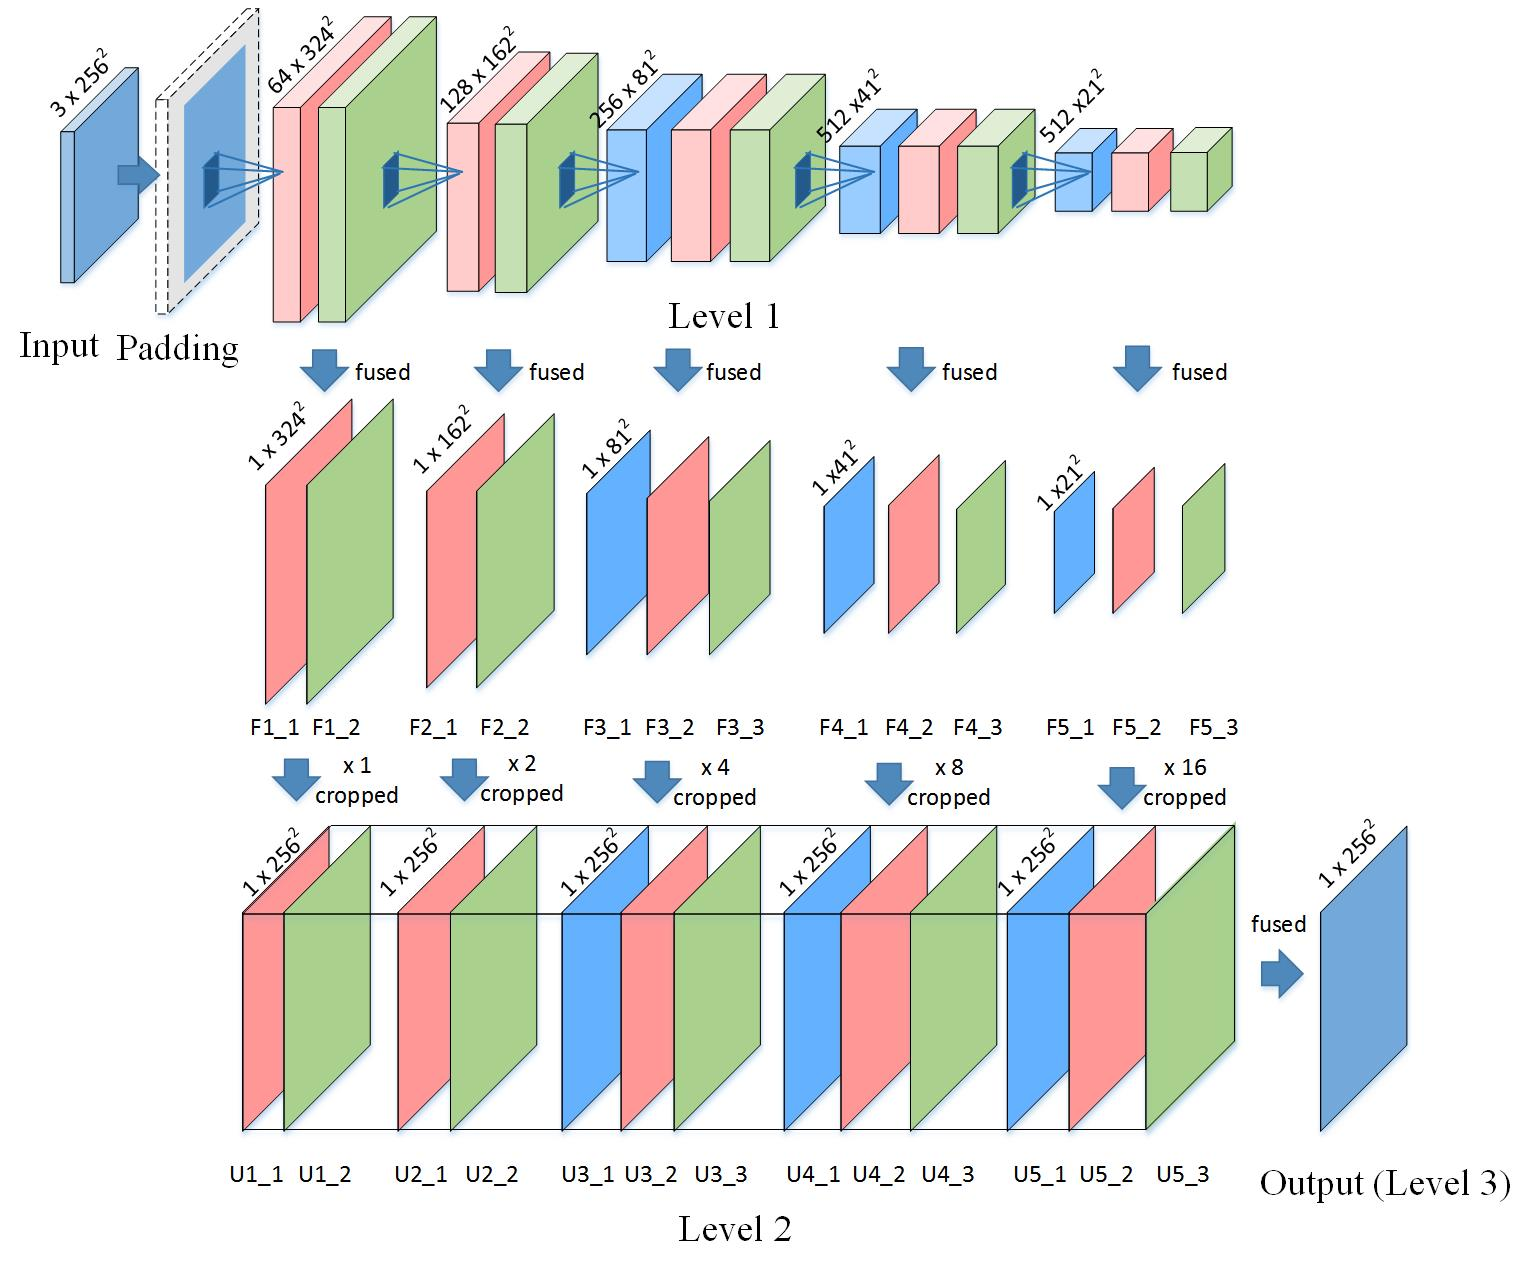
\includegraphics[width=95mm]{figs/hierarchicalFCN-revision}
\caption{Our network architecture. F$1\_1$ means the fusion of feature maps generated from its corresponding convolutional layer conv$1\_1$, U$1\_1$ means the upsampling of F$1\_$1, and so forth.}
\label{fig:hierarchicalFCN}
\end{figure}

   \begin{table}	
	\centering 
	\caption{The receptive field (RF) and the stride size of Level 2 in our architecture.}	
 	\begin{tabular}{C{1cm}|*{16}{C{0.74cm}}} 
	\hline
	layer & F1$\_$1 & F1$\_$2  & F2$\_$1  & F2$\_$2  & F3$\_$1  & F3$\_$2  & F3$\_$3  & F4$\_$1  &   F4$\_$2  & F4$\_$3  & F5$\_$1 & F5$\_$2  &F5$\_$3 \\
	\hline
    RF & 3 & 5  & 10 & 14  & 24  & 32  & 40  & 60  & 76  & 92 & 124  & 164  & 196 \\
	\hline
	stride & 1 & 1   & 2  & 2  & 4  & 4  & 4  &8  & 8  & 8  & 16  & 16  & 16 \\
	\hline
    \end{tabular}
    \label{tab:receptivefield} 
   \end{table}         
    
   In Level 2, the feature maps with increasing receptive field (see Table \ref{tab:receptivefield}) capture local information in larger neighbourhood sizes at higher semantic levels. The shallow layers generate feature maps with fine spatial resolution but low level semantic information. In contrast, the deep layers generate coarse feature maps with high-level semantic information. The feature maps at middle layers correspond to certain intermediate-level features. Integrating all these feature maps, buildings with variant appearances or occlusions are effectively extracted.
  An example is shown in Fig.~\ref{fig:featuremapsofHF-FCN}. Given an aerial image, the U$1\_$1 in Fig. \ref{fig:featuremapsofHF-FCN}(b) with small receptive field extracts low-level features like edges and corners. In Fig.~\ref{fig:featuremapsofHF-FCN}(c), the U1$\_$2 functions like an over-segmentation which groups pixels with similar color or texture into a subregion. 
  In the U2$\_$1 as Fig.~\ref{fig:featuremapsofHF-FCN}(d) shows, shape information is augmented. 
  From the U3$\_$3 as Fig.~\ref{fig:featuremapsofHF-FCN}(e) shows, we can see that regions with significantly varying appearances are merged into an integrated building by considering high-level features. In U4$\_$2 and U5$\_$2 (see Fig.~\ref{fig:featuremapsofHF-FCN}(f)(g)), our network learns strong semantic knowledge to distinguish dark rooftops with dim shadows and dark-green water area. In Level 3, we show that HF-FCN obtains a reliable prediction by combining multi-level semantic information and spatial information, as Fig.~\ref{fig:featuremapsofHF-FCN}(h) shows. 

\begin{figure}
\centering
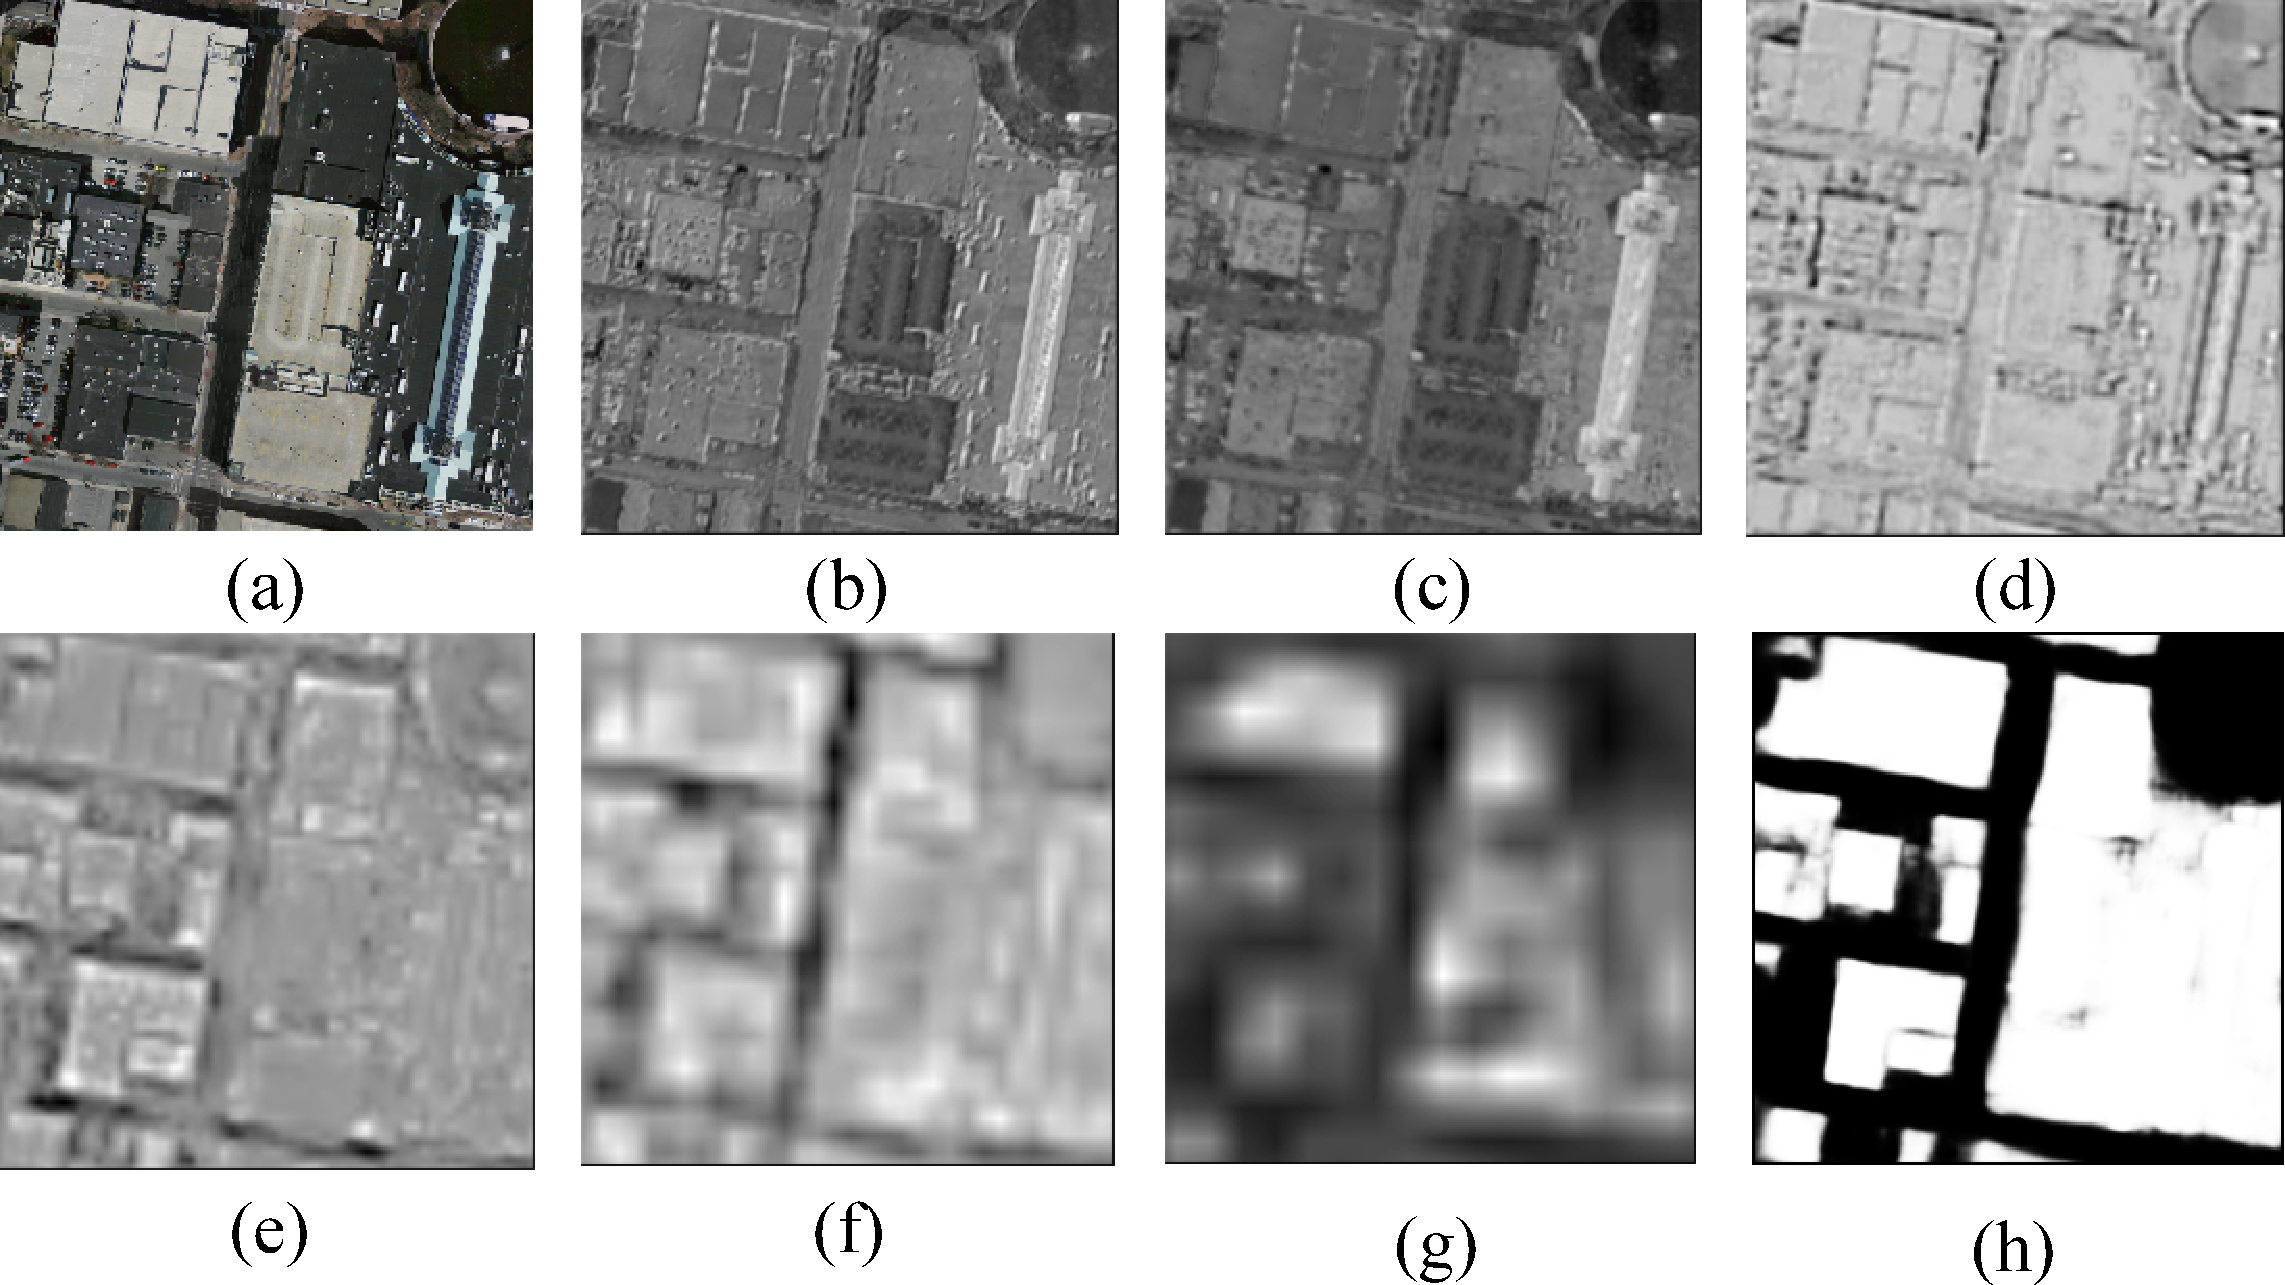
\includegraphics[width=120mm]{figs/featuremaps}
\caption{(a) Input aerial image. (b - g) Feature maps generated from U1$\_$1, U1$\_$2, U2$\_$1, U3$\_$3, U4$\_$2, U5$\_$2, respectively. (h) Predicted labelling map.}
\label{fig:featuremapsofHF-FCN}
\end{figure}

%   In VGG16 Net, 
%   For instance, the first stage generate low level semantic information, such as, regions with similar color or texture, and fine spatial resolution. On the contrary, the last stage outputs strong semantic features but coarse map
%   
%   There are three reasons that FCN-8s is not appropriate methods for building extraction. (1) \textbf{The output of 32 stride layers, including convolutionalized \textit{fc6, fc7} and fifth pooling layer, } (2) The output from FCN-8s is at one-eight of the input resolution. It is not dense enough for very high resolution remote sensing image. Though FCN4s and FCN2s can increase the resolution, they have little help for improving performance. Defective fusion strategy is the most likely reason. On the one hand, in \cite{Long2014Fully}, the coarse predictions from a late stage are upsampled and combined with prediction from its preceding stage using simple sum operation. (3) \textbf{ For instance, in FCN-8s,
%   
% There are two main considerations for choosing hierarchy architecture. Firstly,  buildings especially with large-size have variant appearancess or occlusions.   
   
%\subsection{Architecture Alternatives} 
%In this section, we firstly introduce a well-known semantic segmentation network, called fully convolutional network(FCN)\cite{Long2014Fully}. We attempt to extract footprints of building  using  architecture proposed by author and two modified versions. Our experiments show that these networks are not enough to accomplish building  extraction task. 
%	In our experiments, we first directly apply the FCN-8s to extract building rooftop by replacing the loss function with sigmoid cross-entropy loss. In order to achieving better performance, the network is extended to FCN-4s, FCN-2s. Our experiments show that FCN-4s and FCN-2s get the best performance with overall recall of 70.19 $\%$ in precision recall breakeven point. According to our results, the first row of Fig. \ref{fig:FCN4s-results} indicates that FCN-4s has less ability to handle  objects with small size. The second row of Fig. \ref{fig:FCN4s-results} shows that it is hard for FCN to discriminate buildings with ground if their color is similar. To overcome these drawbacks, a improved FCN is introduced in next section. 
%	
%\begin{figure}
%\centering
%\subfigure[]{	
%	\label{fig:InputImage}
%	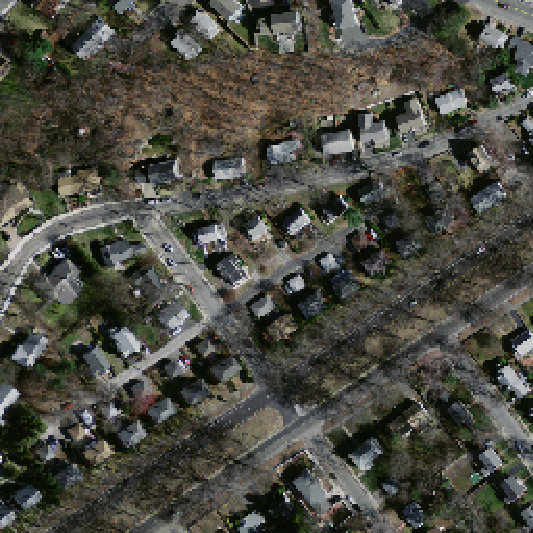
\includegraphics[width=35mm]{FCN4s-results-Input(a)}}
%\subfigure[]{
%	\label{fig:GroundTruth}
%	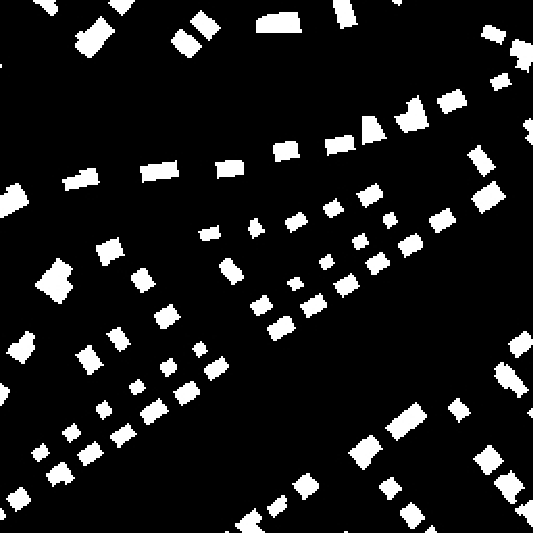
\includegraphics[width=35mm]{FCN4s-results-GT(b)}}
%\subfigure[]{
%	\label{fig:FCN-4s}
%	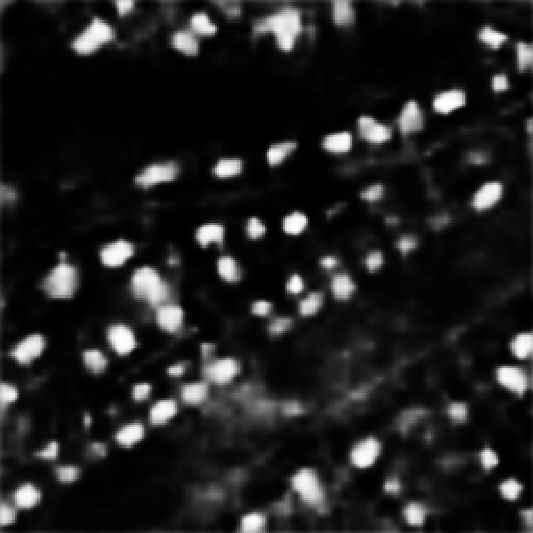
\includegraphics[width=35mm]{FCN4s-results-Prediction(c)}}
%\subfigure[]{	
%	\label{fig:InputImage}
%	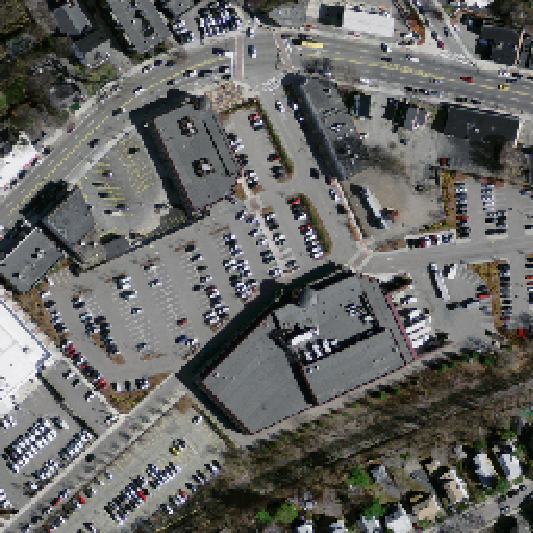
\includegraphics[width=35mm]{FCN4s-results-Input(d)}}
%\subfigure[]{
%	\label{fig:GroundTruth}
%	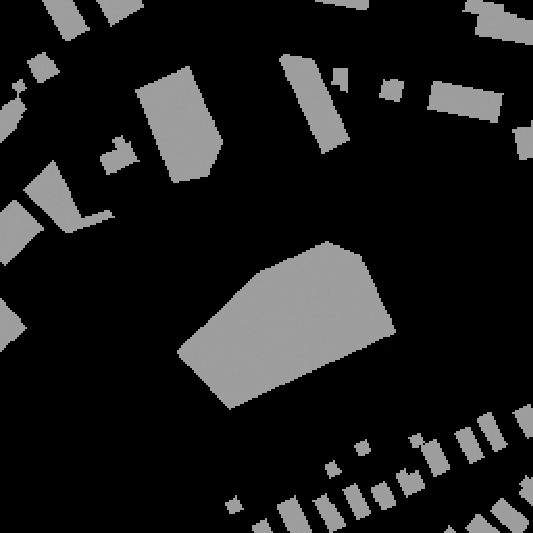
\includegraphics[width=35mm]{FCN4s-results-GT(e)}}
%\subfigure[]{
%	\label{fig:FCN-4s}
%	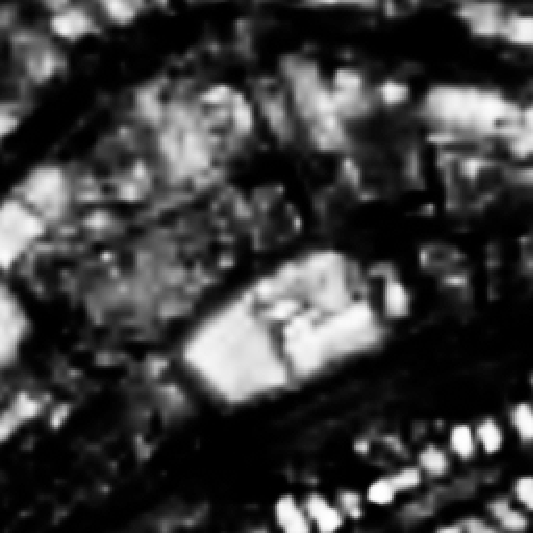
\includegraphics[width=35mm]{FCN4s-results-Prediction(f)}}
%\caption{(a)(d) Input image. (b)(e) Ground truth. (c)(f) FCN-4s prediction.}
%\label{fig:FCN4s-results}
%\end{figure}
% 
        
\subsection{Network Training}
   
 In the training stage, we train our network to directly generate a prediction map $\mathbf{\hat{M}}$ from raw pixels in the input aerial image $\mathbf{S}$ to approach a true label image $\mathbf{\tilde{M}}$. 
 Fig.~\ref{fig:AGroupOfExamples} shows an example of $\mathbf{S}$, $\mathbf{\tilde{M}}$, $\mathbf{\hat{M}}$.  
  %
   We denote our input training data set as $\mathbf{I} = \{(\mathbf{S}_{i},\mathbf{\tilde{M}}_{i}),i = 1,\ldots,N\}$, $N$ is the number of aerial image and labeled map pairs.
% where sample $\mathbf{S}_{n} = \{s_{j}^{(n)}, j = 1,\ldots,\vert \mathbf{S}_n \vert \}$ denotes the raw input image and  $\mathbf{\tilde{M}}_{n} = \{\tilde{m}_{j}^{(n)}, j = 1,\ldots,\vert \mathbf{S_n} \vert\}$, $\tilde{m}_j^{(n)} \in \{0,1\}$ denotes the corresponding ground truth binary labelling map for satellite image $\mathbf{S}_{n}$.  
Taking account of each input image holistically and independently, the subscript $i$ is ignored  for notational simplicity in the following definition. 
In our image-to-image training stage, the loss function is computed over all pixels in a training image $\mathbf{S} = \{s_{j}, j = 1,\ldots,\vert \mathbf{S} \vert\}$ and building map $\mathbf{\tilde{M}} = \{\tilde{m}_{j}, j = 1,\ldots,\vert \mathbf{S} \vert\}$, $\tilde{m}_j \in \{0,1\}$, where $|S|$ is the number of pixels in $\mathbf{S}$.
%
For simplicity, we denote the collection of all standard network layer parameters as $\mathbf{W}$. For each pixel $j$ in a training image, the probability that assigns it to building is denoted as its probability as a building $\hat{m}_j$. 
We use the sigmoid cross-entropy loss function defined as 
\begin{equation}
	\label{loss}
    \mathcal{L} = - \frac{1}{\vert \mathbf{S} \vert} \sum_{s_j \in \mathbf{S}} \left[ \tilde{m}_j \log{\hat{m}_j} + (1 - \tilde{m}_j)\log{(1 - \hat{m}_j)} \right].
\end{equation}

%\begin{figure}
%\centering
%\includegraphics[width=120mm]{AGroupOfExamples}
%\caption{(a) Aerial image $\mathbf{S}$. (b) Ground truth $\mathbf{\tilde{M}}$. (c) Predicted label image $\mathbf{\hat{M}}$. }
%\label{fig:AGroupOfExamples}
%\end{figure}

\begin{figure}
\centering
\subfigure[Aerial image $\mathbf{S}$]{	
	\label{fig:AerialImage}
	\includegraphics[width=38mm]{figs/example-aerialImage}}	
\subfigure[Ground truth $\mathbf{\tilde{M}}$]{
	\label{fig:GroundTruth}
	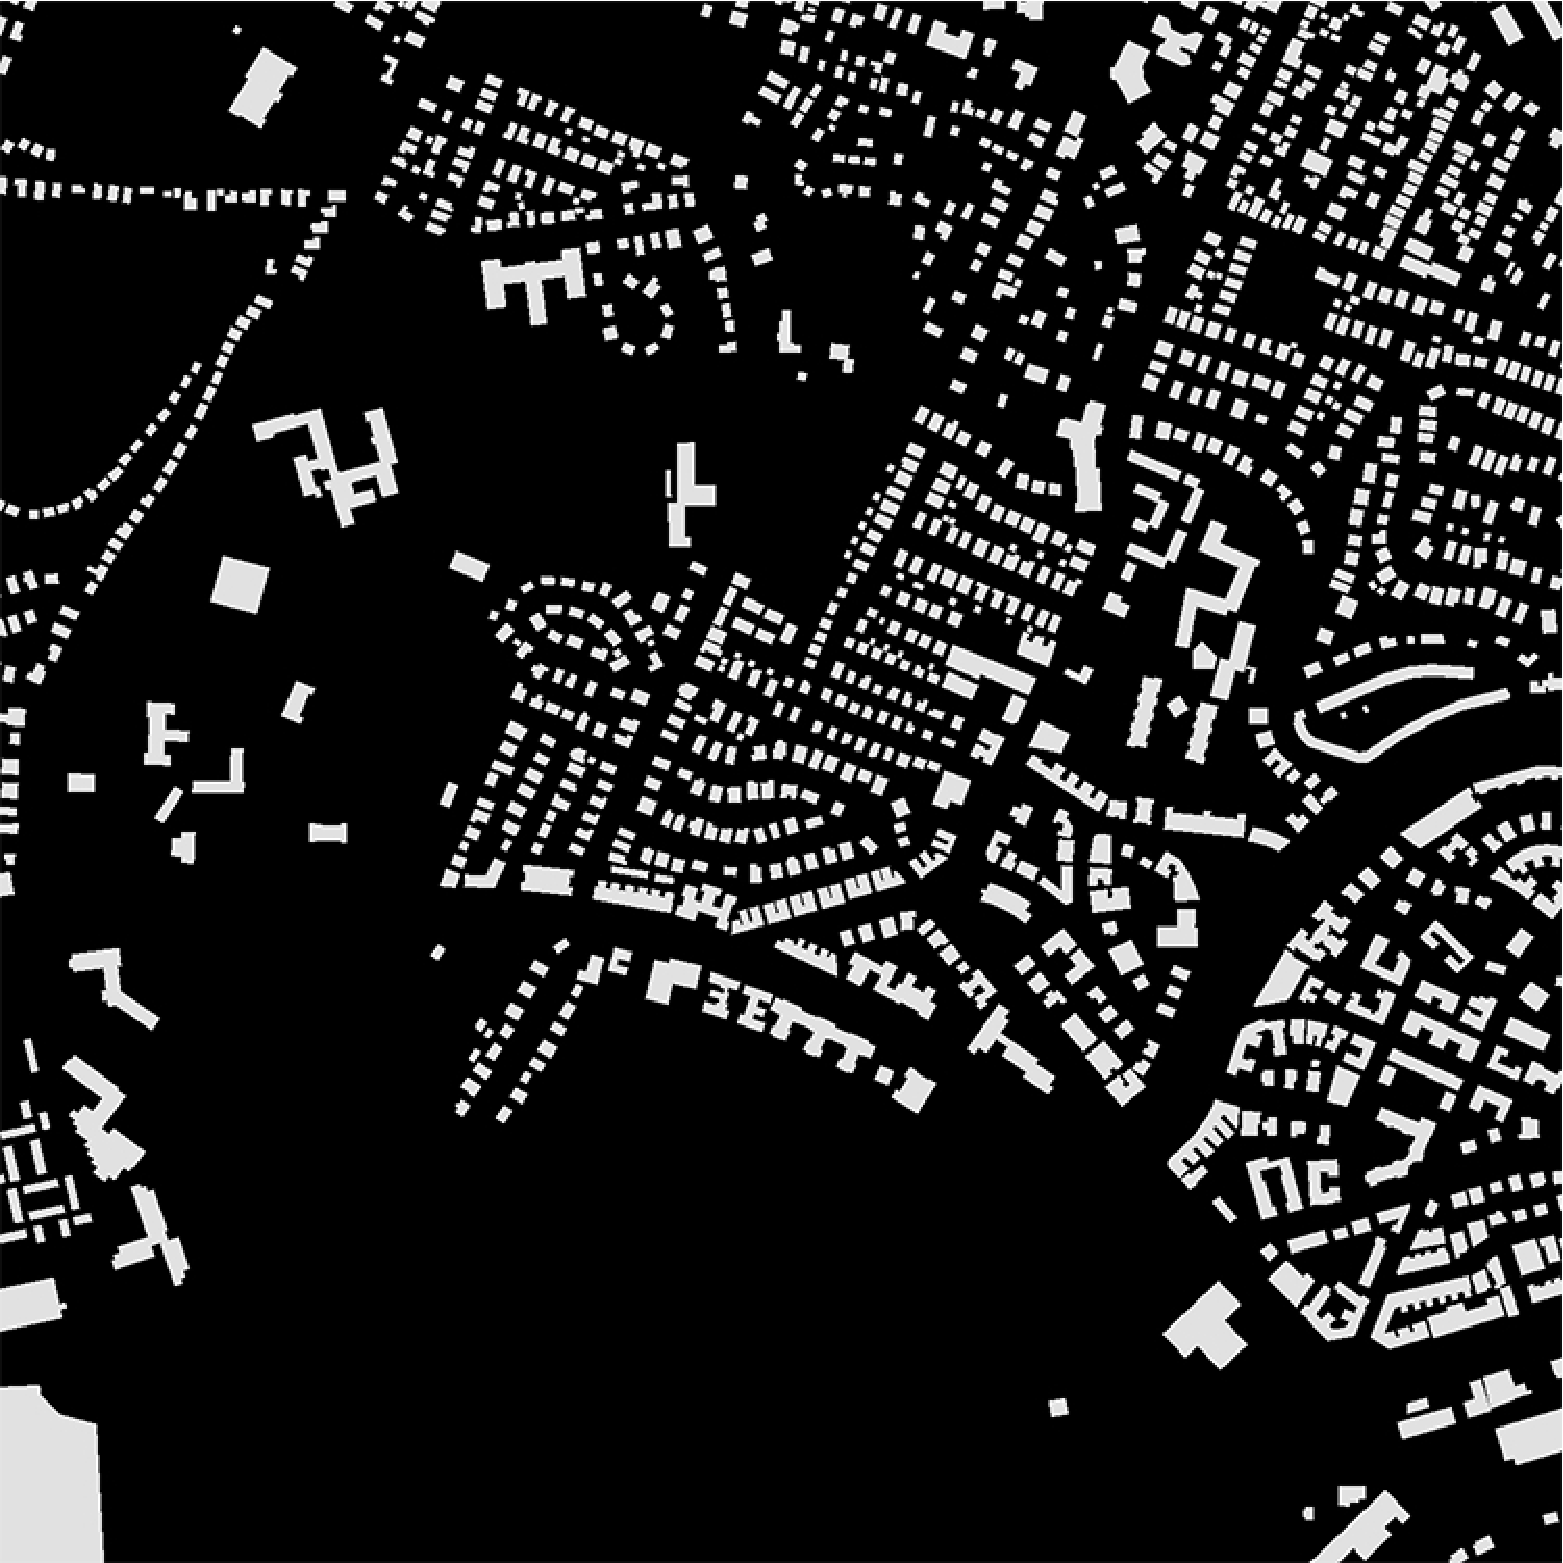
\includegraphics[width=38mm]{figs/example-GT}}	
\subfigure[Predicted image $\mathbf{\hat{M}}$]{
	\label{fig:PredictedResutls}
	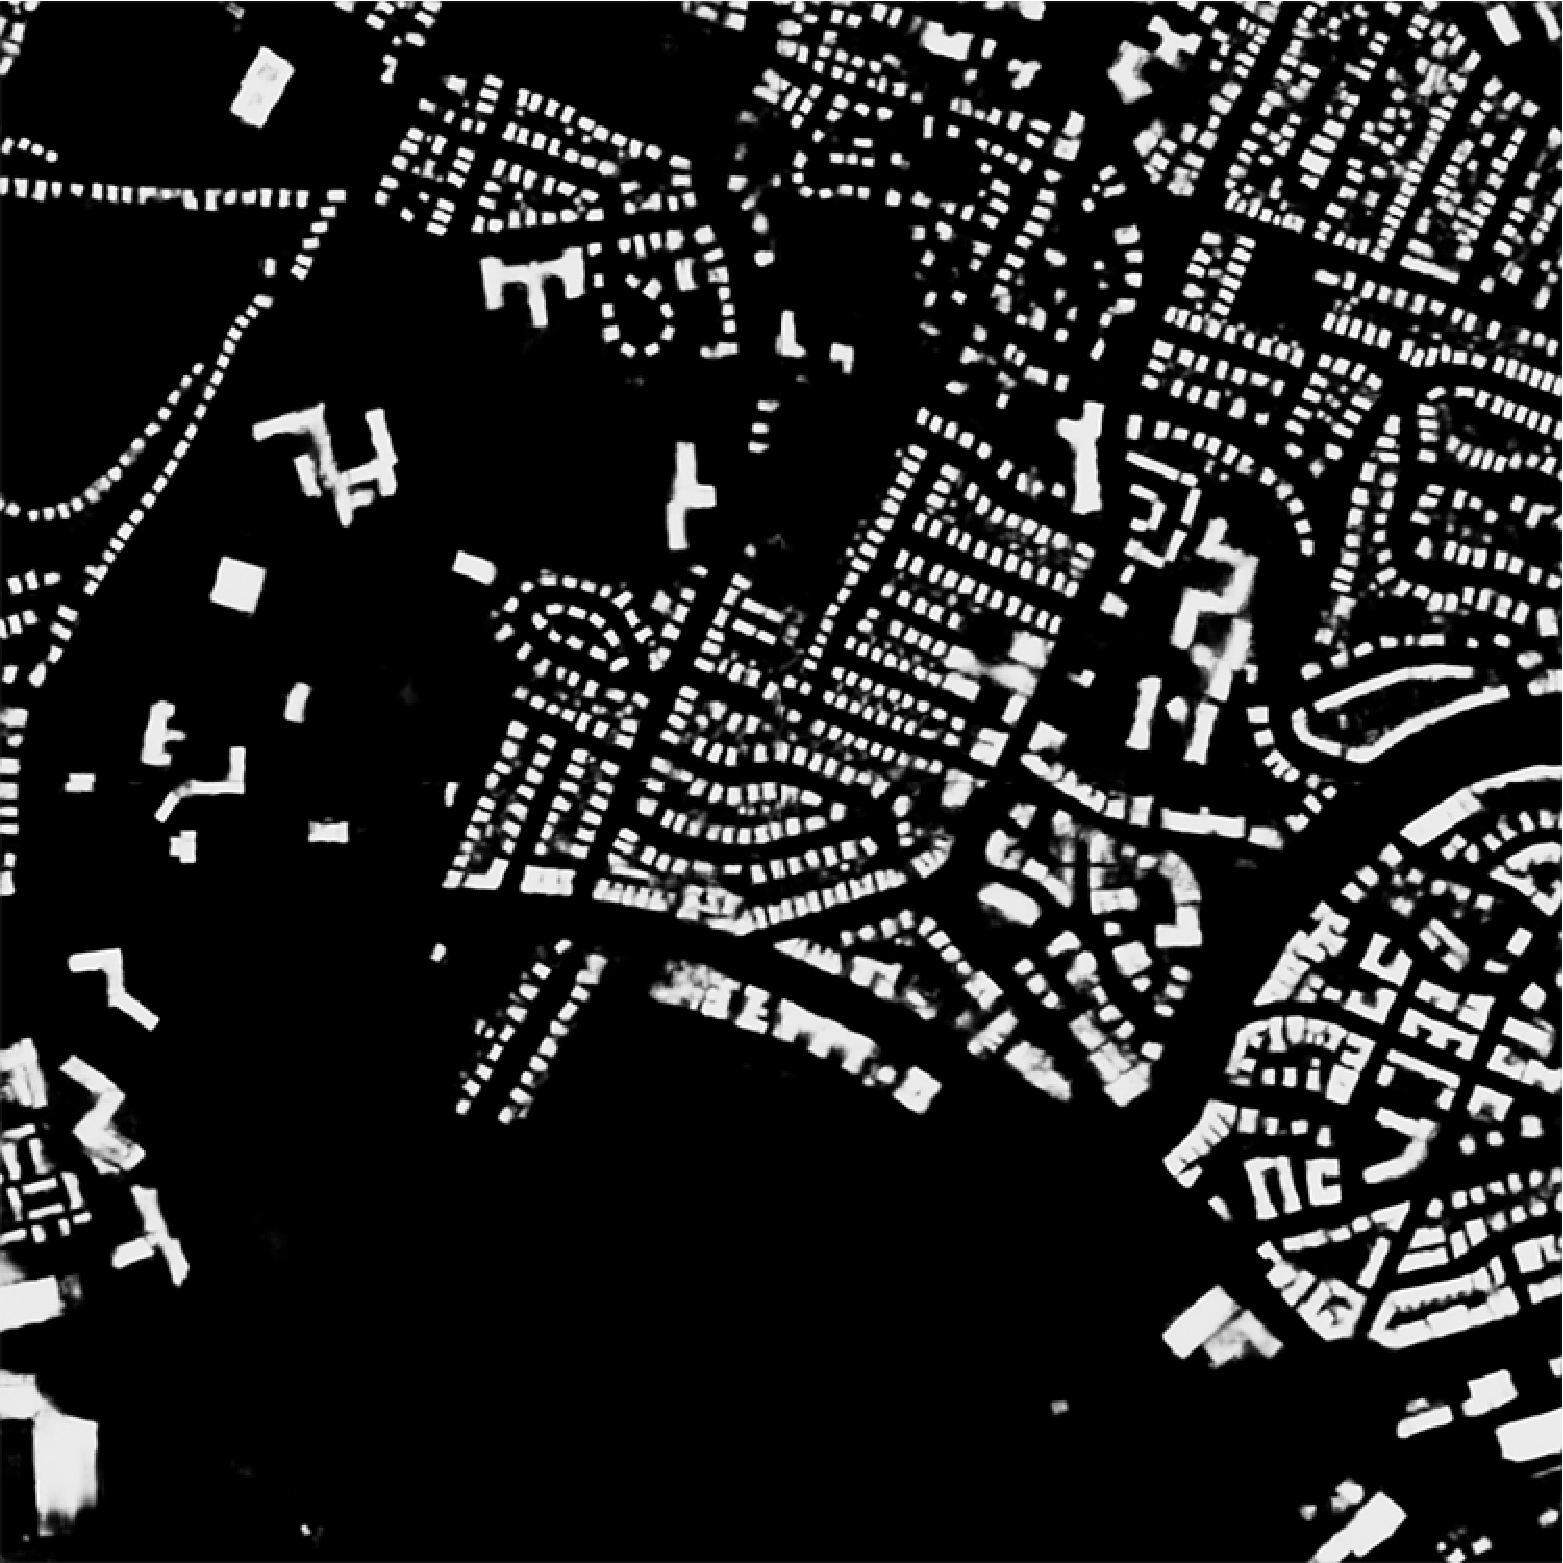
\includegraphics[width=38mm]{figs/example-prediction}}	
\caption{ An example of the resulting predicted image.}
\label{fig:AGroupOfExamples}
\end{figure}



%===========================================================
\section{Experiments}
\label{section:experiments}
In this section, we introduce our detailed implementation and report the performance of our proposed algorithm.

\subsection{Dataset}
  
In our experiments, we use Massachusetts Buildings Dataset (\textit{Mass. Buildings}) proposed by Mnih~\cite{Mnih2013Machine}.
% and publicly available on website \url{http://www.cs.toronto.edu/~vmnih/data/}. 
The dataset consists of 151 aerial images of the Boston area, with each image being 1500$\times$1500 pixels for an area of 2.25 square kilometers. 
The entire dataset covers roughly 340 square kilometers. 
The intensity of each aerial image is scaled into the range of $[0,1]$.
%
The data is split into a training set of 137 images, a test set of 10 images and a validation set of 4 images. 
To train the network, we create a set of image tiles for training and validation by cropping each aerial image using a sliding window with size of 256$\times$256 pixels and stride of 64 pixels.
%
 After scanning, the training and validation datasets include 75938 tiles and 2500 tiles respectively, with their corresponding building masks. 
For testing, we use ten 1500$\times$1500 images excluded from the training images.
%  

\subsection{Training Settings}
 
The implementation of our network is based on the \textit{Caffe}  Library~\cite{Jia2014Caffe}. Our HF-FCN is fine-tuned from an initialization with the pre-trained VGG16 Net model and trained in an end-to-end manner. It is trained using the stochastic gradient descent algorithm, with the hyper-parameters listed in Table~\ref{tab:paramerters}. 
%
The learning rate is divided by 10 for each 8000 iterations.
We find that the learned deconvolutions provide no noticeable improvements in our experiments, similar as \cite{Long2014Fully,Holistically2015}. Therefore, lr$\_$mult is set to zero for all deconvolutional layers.  
%
Except that the pad of first convolutional layer is set to 35, the others are set to 1, same as VGG16 Net. 
%
It takes about six hours to train our network on a single NVIDIA Titan 12GB GPU.
\begin{table}
	\centering
	\caption{Parameters for network training.}
		\begin{tabular}{r|c}
		\hline
		mini-batch size & 18 \\
		initial learning rate & $10^{-5}$\\
		momentum & 0.9\\
		weight decay & 0.02\\
		clip$\_$gradients & 10000 \\
		the number of training iterations & 16000\\		
		\hline
		\end{tabular}
	\label{tab:paramerters} 
\end{table}


\subsection{Results}
 
To show the effectiveness of HF-FCN, we compare our method with two state-of-the-art approaches~\cite{Mnih2013Machine,Saito2016Multiple}.
Three common metrics are used to evaluate the performance of our algorithm: (1) the relaxed precision and recall scores with $\rho = 3$; (2) the standard precision and recall scores ($\rho= 0$); (3) the time cost.  
The relaxed precision is defined as the fraction of detected pixels that are within $\rho$ pixels of a true pixel, while the relaxed recall is defined as the fraction of the true pixels that are within $\rho$ pixels of a detected pixel.
%
The slack parameter $\rho$ is set to 3, which is the same value as used in \cite{Mnih2013Machine,Saito2016Multiple}. 
The relaxed precision-recall curves generated from different methods are shown in Fig.~\ref{fig:relaxedcurve}. As can be seen, all curves of ours are located above others in building prediction obviously.
%
More strictly, we set slack parameter $\rho$ as 0, that is to say, it becomes a standard precision and recall scores. 
%
The precision-recall curves generated from different methods are shown in Fig.~\ref{fig:standardcurve}. We can see that our approach is more appropriate for detecting rooftops in complex scene,  which significantly outperforms  \cite{Mnih2013Machine,Saito2016Multiple}.
%
To compare the system efficiency, we calculate the average time of processing ten test images in the same computer using different methods. 
Table~\ref{tab:PerformanceComparision} shows that our method is able to not only significantly improve the performance, but also dramatically reduces the time cost. 
      
\begin{figure}
\centering
\subfigure[Slack parameter $\rho$ = 3]{	
	\label{fig:relaxedcurve}
	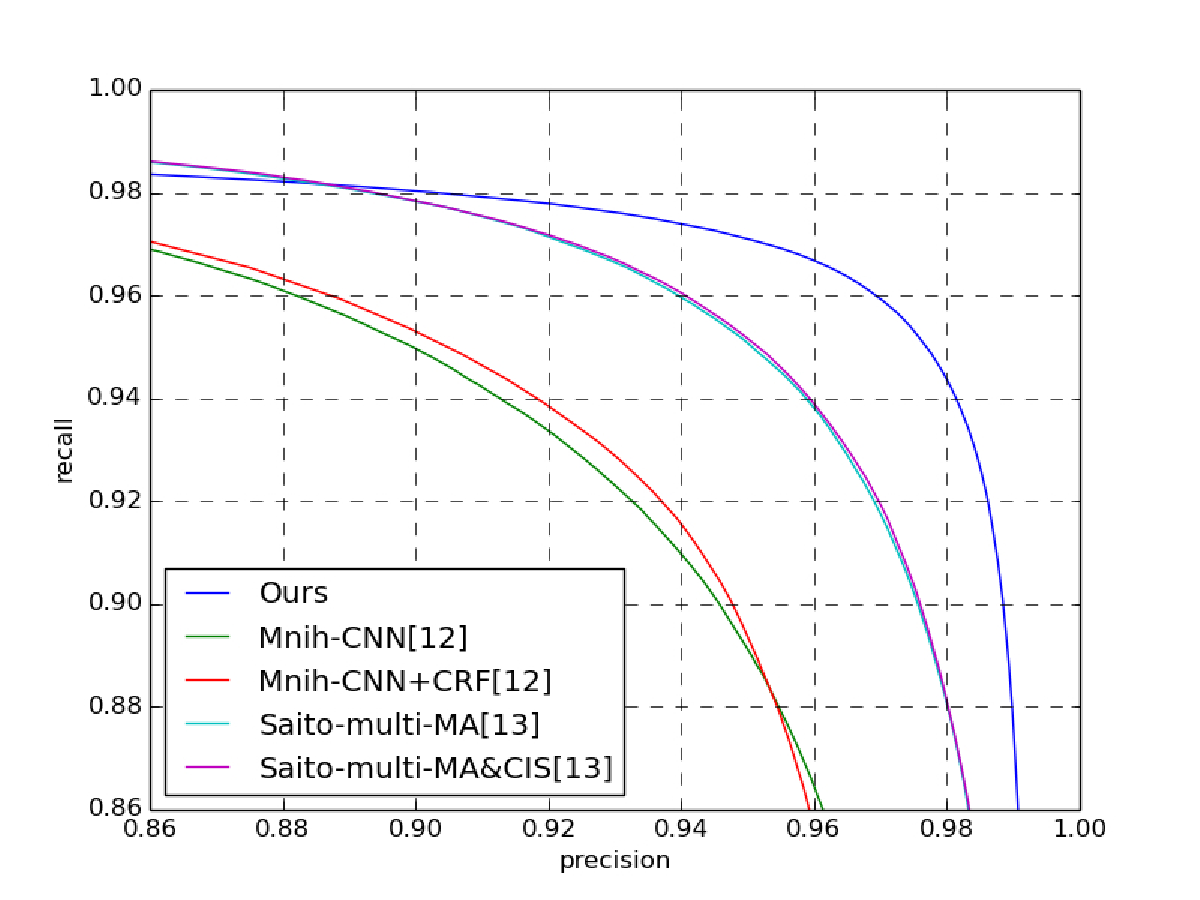
\includegraphics[width=59mm]{figs/PrecisionRecallCurve_3}}
\subfigure[Slack parameter $\rho$ = 0]{
	\label{fig:standardcurve}
	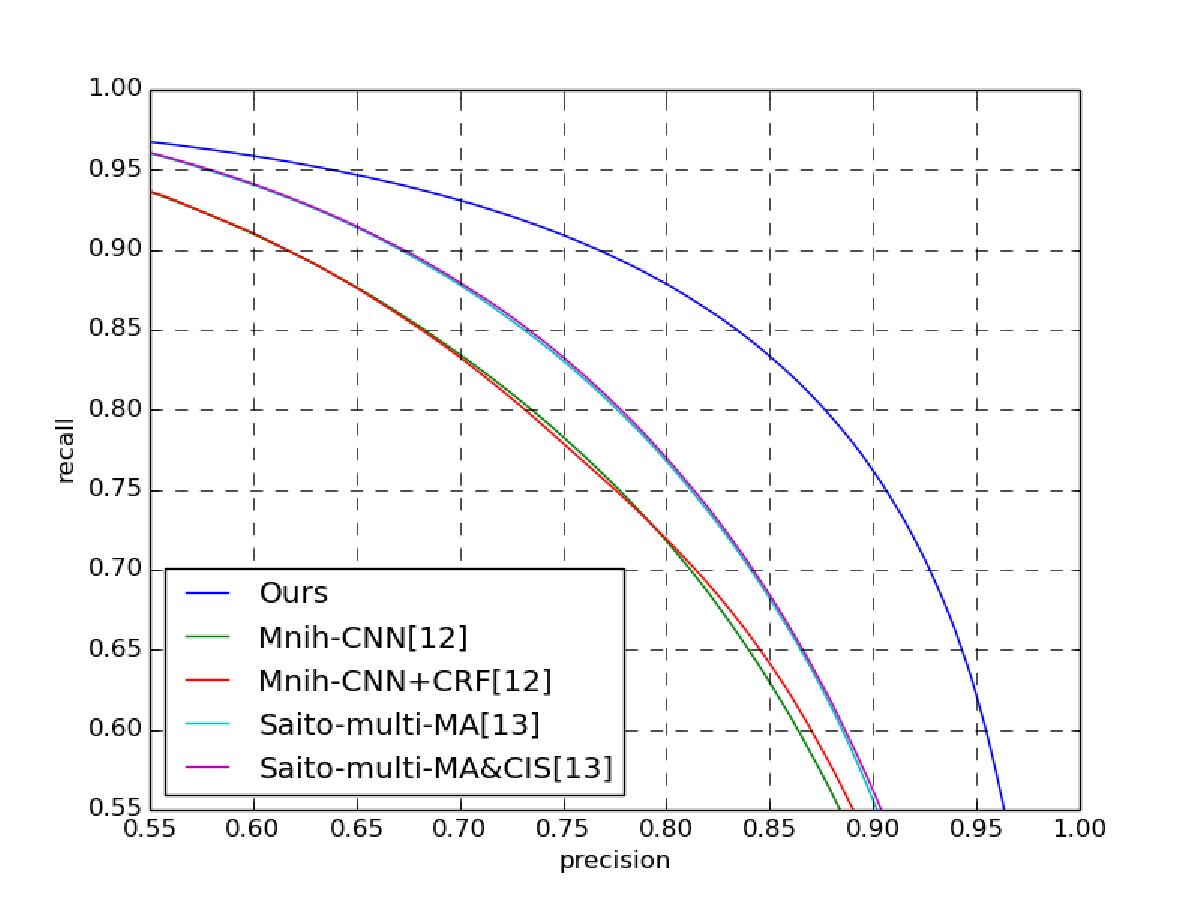
\includegraphics[width=59mm]{figs/PrecisionRecallCurve_0}}
\caption{The relaxed precision-recall curves from different methods with two slack parameters.}
\label{fig:}
\end{figure}
 
    \begin{table} 
    \centering
	\caption{Performance comparison with \cite{Mnih2013Machine,Saito2016Multiple}. Recall here  means recall at breakeven points. Time is computed in the same computer with a single NVIDIA Titan 12GB GPU.}
	\begin{tabular}{L{38mm}C{26mm}C{26mm}C{26mm}}     
	\toprule
	& Recall ($\rho$ = 3) & Recall ($\rho$ = 0)& Time (s)\\
	\midrule
	Mnih-CNN \cite{Mnih2013Machine} & 0.9271 & 0.7661 & 8.70  \\ 
	Mnih-CNN+CRF \cite{Mnih2013Machine} & 0.9282 & 0.7638 & 26.60\\ 
	Saito-multi-MA \cite{Saito2016Multiple} & 0.9503 & 0.7873 & 67.72 \\
	Saito-multi-MA$\&$CIS \cite{Saito2016Multiple} & 0.9509 & 0.7872 & 67.84 \\
	Ours (HF-FCN) & $\bm{0.9643}$ & $\bm{0.8424}$ & $\bm{1.07}$\\
	\bottomrule
	\end{tabular}
	\label{tab:PerformanceComparision}
	\end{table}  
 
 	 
\begin{figure}
\centering
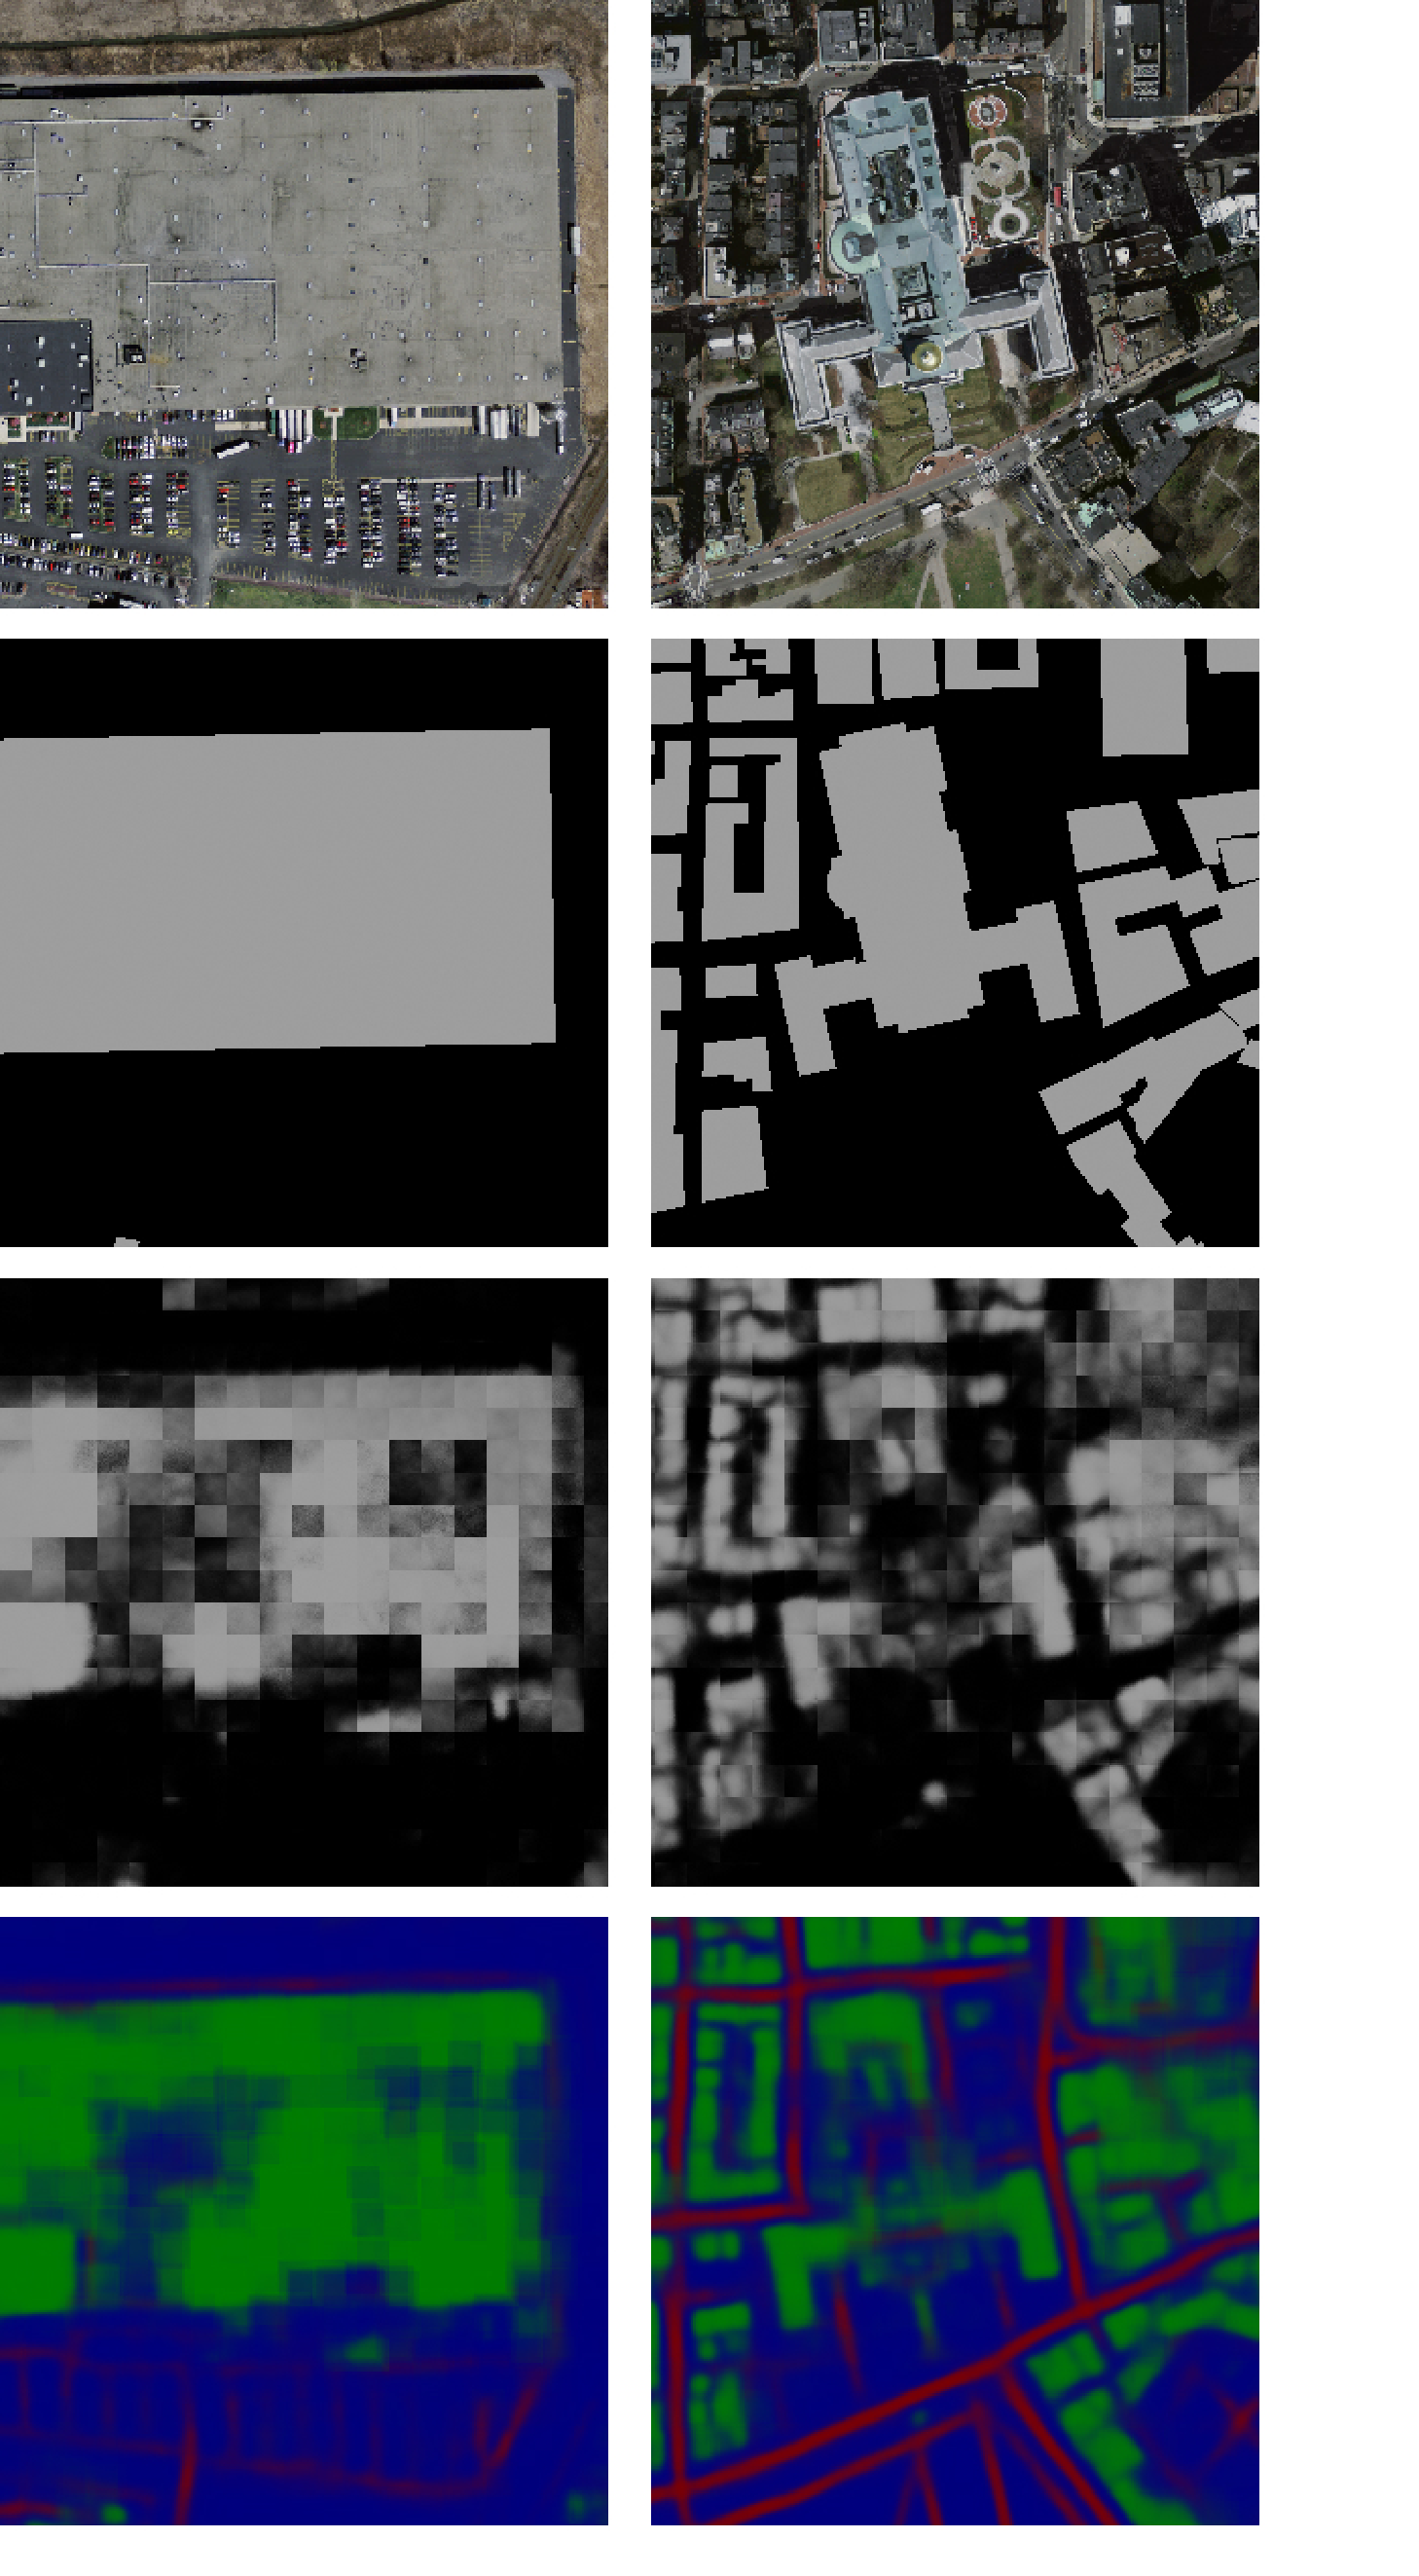
\includegraphics[width=110mm]{figs/ComparedResults}
\caption{(a) Input images. (b) Results of Mnih-CNN+CRF \cite{Mnih2013Machine}. (c) Results of Saito-multi-MA$\&$CIS \cite{Saito2016Multiple}. (d) Our results. 
Correct results (TP) are shown in green, false positives (FP) are shown in blue, and false negatives (FN) are shown in red.}
\label{fig:ComparedResults}
\end{figure} 
    
 
To prove that our network has strong ability in extracting buildings with variant appearances, arbitrary sizes, occlusions, a new experiment is designed.
% 
We crop seven 256$\times$256 image patches that have buildings with variant appearances or occlusions from the test images. 
Corresponding predictions are directly  cropped from the predicted images generated by three approaches, including Mnih-CNN+CRF~\cite{Mnih2013Machine}, Saito-multi-MA$\&$CIS~\cite{Saito2016Multiple} and ours. 
We binarize the probability map using a threshold of 0.5. A series of examples is shown in Fig.~\ref{fig:ComparedResults}.
%
In addition, Table~\ref{tab:ComparedResultsRecall} shows the resulting recalls at the breakeven points of the standard precision recall curve for each patch. The accuracy of our approach is 12.7\% , 6.0\% higher than \cite{Mnih2013Machine},\cite{Saito2016Multiple}, receptively.
 

	\begin{table} 
    \centering
	\caption{Recall at the selected regions of the test images.}
	\begin{tabular}{L{38mm}*{9}{C{9mm}}}     
	\toprule
	Image ID & 01 & 02 & 03 &04 &05 & 06 &07 & mean\\
	\midrule
	Mnih-CNN+CRF~\cite{Mnih2013Machine} & 0.784 & 0.869 & 0.769 & 0.653 & 0.893 & 0.764 & 0.800 & 0.784\\
	Saito-multi-MA$\&$CIS~\cite{Saito2016Multiple} & 0.773 & 0.915 & 0.857 & 0.789 & 0.945 & 0.773 &0.830 & 0.851\\
	Ours (HF-FCN) & $\bm{0.874}$ & $\bm{0.964}$  & $\bm{0.899}$ & $\bm{0.901}$ & $\bm{0.986}$ & $\bm{0.840}$ &  $\bm{0.851}$ & $\bm{0.911}$\\
	\bottomrule
	\end{tabular}
	\label{tab:ComparedResultsRecall}
	\end{table} 
 	 
   

%===========================================================
\section{Conclusions}
\label{section:conclusions}
   In  this article, we propose a novel fully convolutional network which is  strongly capable of extracting buildings of arbitrary sizes, variant appearances or occlusions without any post-processing. Meanwhile, it further improves the overall accuracy. The proposed network can take arbitrary-size image as the input as long as the GPU memory allows. Compared with patch-based methods, there is no need to label a whole image by cropping the image into small patches. As consequence, inconsistent border caused by cropping would not occur in our system. Moreover, the time cost is tremendously reduced using our HF-FCN. 
   The proposed method is demonstrated robust to various types of aerial scenes selected from real-world data. Furthermore, our architecture can be easily extended to extract multi-objects in remote sensing imagery. 
   Consequently, we believe that our technique potentially provides a generic solution to understand complex aerial scenes.
	
%HF-FCN provides a strong ability to extracting building rooftops even with significantly variant appearancess and severely occlusions   Meanwhile, it further improves the overall accuracy than \cite{Mnih2013Machine}\cite{Saito2016Multiple}. Compared with patch based methods \cite{Mnih2013Machine}\cite{Saito2016Multiple}, HF-FCN takes whole images as inputs without cropping or warping them to a fixed size and directly outputs segmentation maps by one pass of forward propagation. 
%===========================================================
\bibliographystyle{splncs}
\bibliography{hf-fcn}

%this would normally be the end of your paper, but you may also have an appendix
%within the given limit of number of pages
\end{document}
